\documentclass[12pt,a4paper]{article}

\usepackage[utf8]{inputenc}
\usepackage[spanish]{babel}
\usepackage[T1]{fontenc} 
\usepackage{graphicx} 
\usepackage{geometry} 
\geometry{margin=2.5cm}
\usepackage{listings}
\usepackage{xcolor}
\usepackage{hyperref}
\usepackage{tikz}
\usepackage{adjustbox}
\usetikzlibrary{positioning, arrows.meta}
\usepackage{graphicx}
\addto\captionsspanish{%
  \renewcommand{\abstractname}{Abstract}
}
\title{Reporte Base de Datos Musical}
\author{Jesus Figueroa Ramirez} 
\date{\today}

\begin{document}
\begin{titlepage}
    \centering
    {\LARGE \textbf{Universidad Nacional Autónoma de México} \par} 
    \vspace{0.5cm}
    {\Large \textbf{Facultad de Ciencias} \par}
    \vspace{3cm} 
    {\Huge \textbf{Base de datos musical} \par}
    \vspace{1cm}
    {\Large Reporte de proyecto \par}
    \vspace{4cm}
    {\Large Presenta: \par}
    \vspace{0.5cm}
    {\Large \textbf{Jesus Figueroa Ramírez} \par} 
    \vfill 
    {\large Ciudad de México \par} 
    {\large \today \par}
    
\end{titlepage}
    

\begin{abstract}
This project focuses in the implementation of local musical database. Using the Rust Programming language
and the Slint UI Framework to make a very fast and cross platform app. The result shows that 
using this framework with rust can lead to a very fast implementation and good results even for low
resources hardware.
\end{abstract}

\section{Introducción}
Este proyecto de presenta como un primer acercamiento a el manejo de bases de datos, la minería de datos, 
un pseudo compilador y el diseño de interfaces gráficas, todo esto con las mejores prácticas de programación
y los paradigmas adecuados para cada problema. En este caso se opto por desarrollar la funcionalidad 
del programa con el lenguaje Rust debido a la familiaridad con el mismo y su eficiencia para manejar
operaciones como la minería y el compilador de una forma bastante eficiente. Durante el desarrollo se 
considero utilizar GTK4 en lugar de Slint para desarrollar la interfaz sin embargo se decantó por Slint 
debido a que era una herramienta multiplataforma y ligera, además su sintaxis permitía que su curva de 
aprendizaje fuera menor a la otra opción.

\section{Objetivos}
\subsection{Objetivo General}
Desarrollar una aplicación de base de datos musical en local.
\subsubsection{Objetivos específicos}
\begin{itemize}
  \item Interfaz de usuario mediante la cual el usuario pueda modificar aspectos de la base de datos y 
    realizar búsquedas.
  
  \item Compilador con el cual se permite que el usuario realice búsquedas sin necesidad
    de escribir sql para realizarlo.
  
  \item Un minero que permita extraer todos los datos de los archivos mp3 de una ruta raíz dada por el usuario.
  
  \item Utilizar el patrón de diseño DAO para interactuar con la base de datos sin necesidad de 
    escribir sql constantemente en todo el programa.
\end{itemize}


\section{Desarrollo}
Al inicio del proyecto se decidió utilizar rust debido a que era la herramienta más familiar de desarrollo 
además de que es una herramienta muy buena en cuanto a rendimiento lo cual sería de utilidad al realizar 
la minería, el compilado del lenguaje de búsquedas y las peticiones a la base de datos.

En cuanto a las herramientas para el diseño de la interfaz gráfica si bien se optó por Slint como la herramienta
a utilizar, se consideraron múltiples opciones para la misma, en principio lo más natural fue pensar en GTK4 como
la herramienta por excelencia para desarrollar apps para linux, sin embargo su sintaxis no era de lo más agradable
, aún con ello fue la opción más fuerte en un inicio, se consideraron otras opciones, entre ellas el framework Iced,
sin embargo al final solo había dos opciones viables, SLint y GTK.

Slint es una herramienta relativamente nueva, muy útil para interfaces ligeras ya que esta pensada para su uso en 
sistemas embebidos, además por como realiza el renderizado de la interfaz, es completamente multiplataforma y 
su lenguaje para describir interfaces gráficas es bastante amigable. Por otra parte está GTK4, una opción 
muy potente y madura, nativa en linux y creada para ello, sin embargo debido a las particularidades de Rust
el utilizar GTK lleva ciertas complicaciones que sumadas a el tiempo limitado de desarrollo
hicieron que Slint fuera la opción más viable para este proyecto.

El desarrollo inició por la parte del minero, esta parte fue particularmente veloz debido a una biblioteca llamada WalkDir
que realizaba el recorrido de un directorio de forma recursiva extrayendo cualquier archivo y directorio, gracias a esta 
herramienta ya se contaba con una parte muy importante del minero que era extraer todo lo que hubiera desde el directorio 
raíz elegido, entonces el trabajo continuaba por filtrar lo que se encontrara en todo ese directorio, como solo eran necesarios
los archivos mp3 el primer filtro fue eliminar todas las referencias a los directorios las cuales no serían necesarias,
después filtrar por archivos con extensión mp3 ya que el resto no era de nuestro interés, con ello obteniamos todos los archivos mp3
en el directorio dado, ahora es necesario procesar cada uno de estos archivos, primero verificamos que sea posible 
obtener su dirección absoluta en memoria ya que esto sería útil más adelante al extraer imágenes o el audio mismo, 
de no estar disponible se procedía a descartar el archivo, pasado este filtro se verificaba que la etiqueta del
archivo mp3 correspondía al tipo id3v2.4 de otra manera también se descartaba, por último se extraían los datos 
escritos en esta etiqueta proveyendo datos por defecto en caso de no existir alguno para así mantener consistencia
en los mismos, todos estos datos se almacenaban en una estructura para ello y se retornaba un vector con los datos
de cada canción.

El siguiente paso natural es crear la base de datos para poder guardar los datos que es extrajeron, en este caso
esto se realizaría en el dao, primero se define una constante con los comandos para definir la estructura de la base de datos
, con ello se define el dao que con una ruta abre una conexión a la base de datos en esa ruta en caso de existir o la crea en 
otro caso, después verifica que la estructura corresponda con la deseada o si no la elimina y crea una nueva que si cumpla con 
la estructura. Esto llevo a un problema al implementar búsquedas al final del proyecto, ya que por como estaba definido 
el método que verificaba la estructura llevaba a que siempre que se instanciaba un dao la base de datos se eliminara y se 
volviera a crear borrando los datos en ella, después de buscar el error por horas en el minero, compilador o en como se devolvían
las canciones para la interfaz, se encontró que el problema estaba aquí por lo cual al final solo se verifica que exista la tabla 
principal Rolas y se supone que si existe es por que la base de datos corresponde a lo esperado.

El siguiente paso es definir el método para poder insertar canciones en la base de datos, este método llamado 
naturalmente insert-songs recibe un vector con los datos de las canciones y se encarga de insertarlas a la base de datos
verificando ciertas cosas como si ya existía previamente la canción, además llena el resto de las tablas con estos mismos datos
como corresponde en cada caso.

Por último se definió un método para extraer estas canciones de la base de datos en una estructura que obtuviera los datos
necesarios para la interfaz gráfica.

Con lo anterior implementado y sus pruebas respectivas el siguiente paso fue definir la interfaz para poder visualizar
estos datos, en un principio se diseñó tomando en cuenta el reproductor sin embargo este no fue incluido en la versión de entrega 
por falta de tiempo, así que gran parte de lo realizado en este periodo no se incluyo en la entrega o fue refactorizado básicamente
en su totalidad, sin embargo este periodo fue importante para aprender sobre los elementos en Slint y como funcionaban así 
para aprender sobre los callbacks y como utilizarlos y definirlos.

Paso un gran periodo de tiempo en el desarrollo de lo mencionado anteriormente a lo que se describirá a continuación
debido a múltiples factores. Una vez retomado el proyecto debido a el poco tiempo restante de desarrollo lo que continua 
fue desarrollado de forma bastante caótica, primero se inició con la investigación de como desarrollar el compilador de búsquedas y 
las herramientas necesarias, se encontró una biblioteca llamada pest la cual permitía definir la gramática de nuestro lenguaje 
para entregarnos las partes correspondiente y ahorrar tiempo haciendo esto manualmente, con ello se definió el lenguaje y se 
define su gramática en un archivo .pest para que se pueda utilizar en rust, se define un enumeración para poder definir el árbol 
ast con base en lo entregado por pest, en donde a cada tipo definido en la gramática se asigna un tipo en la enumeración, se define un método 
asociado a esta enumeración que toma lo entregado por pest y recursivamente lo traduce a la enumeración para tener un objeto que represente la búsqueda.
Por último se crea un método público que recibe una cadena y obtiene el árbol ast expresado directamente en esta enumeración o devuelve 
un error si la cadena no corresponde con la gramática definida.

Una vez teniendo el árbol ast es necesario obtener el texto sql del mismo, para ello se crea un estructura llamada sql-query la cual
se encarga de mantener la cadena sql que se tiene el momento y los parámetros correspondientes para cada petición. El método 
que genera la cadena sql funciona de la siguiente manera, descifra cada cadena recursivamente usando como condición base 
una condición sencilla del tipo <<artista = algo>> esto corresponde al tipo de la enumeración Condition que tiene un valor y un campo, entonces
se verifica que el campo corresponda a uno de los campos de búsqueda y se traduce en caso exitoso al campo correspondiente en la tabla Rolas
, se utiliza un place holder "= ?" para evitar la inserción de sql y se añade el valor al vector de parámetros, después estas condiciones bases 
se utilizan para formar el resto de condiciones, por ejemplo en el caso anterior tenemos la cadena <<artista = ?>> como el código sql y <<algo>> como
el único parámetro, si esta condición se encontrara dentro de una expresión de negación entonces se genera la cadena <<NOT ()>> y se inserta el código
sql obtenido anteriormente dentro de paréntesis y como en este caso la lista de parámetros no se ve afectada solo tendríamos como parámetros <<algo>>, en
el caso en donde se añaden parámetros se añadiría <<algo>> al final de la lista de nuevos parámetros. De esta forma se obtiene la cadena sql
pudiendo realizar peticiones con condiciones arbitrarias.

Por último en el dao se define un método que toma un árbol ast y realiza la búsqueda, primero compila el ast a sql y después define de donde 
se van a obtener esos datos en la base de datos y los joins necesarios para añadir la cadena sql generada y con la lista de parámetros poder realizar
la consulta devolviendo un vector con los datos de las canciones que cumplen con la búsqueda.

En este punto se tenía definida la vista en forma de lista en la interfaz que sería lo único que se rescataría 
de forma parcial de todo el trabajo en la interfaz realizado anteriormente. Debido al corto tiempo disponible 
para el desarrollo en ese momento se optó por tomar esta base y simplemente definir la forma de vista en el mismo 
componente para así poder aprovechar todos los callbacks y datos de entrada ya definidos, aunque esto no es una
buena práctica fue necesario por cuestión de tiempo.

Por último quedaba conectar todo el trabajo que se realizaba en Rust para poder mostrarlo en la interfaz, se definió
una clase controller para manejar todo esto, primero se pensó que el controlador tuviera un dao asignado para realizar todas
las operaciones con la base de datos sin embargo al manejar hilos de ejecución no era seguro mandar un objeto de este tipo a través 
de ellos, entonces la mejor opción fue simplemente guardar la dirección de la base de datos para poder generar un dao cada que fuera
necesario interactuar con la base de datos, así mismo el controlador también guarda una referencia débil a el manejador de la
interfaz para poder actualizarla cuando sea necesario. Este controlador tiene métodos para responder a los callbacks de la interfaz,
al recibir un directorio para minar toma la ruta e inicia el minado para insertar los datos en la base de datos y extraerlos para 
inmediatamente después mostrarlos, está función siempre solicita de nuevo la lista actualizada de canciones así se obtiene todas las canciones
que han sido minadas, pudiendo así llenar con datos de distintos directorios la base de datos y poder reunirlos en la base de datos.

También se encarga de responder a cuando la interfaz solicita una búsqueda, llama a los métodos necesarios y en caso de error no realiza nada,
y en caso contrario devuelve un vector con los resultados de la búsqueda. En este sentido faltó alguna forma de volver a mostrar las canciones en 
general después de realizar una búsqueda.

También se implemento el método para actualizar los datos del artista en la base de datos sin embargo faltó implementar esto mismo 
pero para los grupos o bandas.

Al terminar se puede notar que puede que el proceso desde minar o realizar una búsqueda sea lento, esto no es debido al minero o las consultas 
sino que para poder renderizar las imágenes se deben extraer los datos del tag que es una operación lenta y faltó implementar esto adecuadamente
para que la interfaz no se ralentice en lo que se obtienen las imágenes.

\begin{figure}[h]
    \centering
    \begin{adjustbox}{max width=\textwidth}
    \begin{tikzpicture}[
        node distance=1.2cm and 1.5cm,
        umlbox/.style={
            draw, thick, rounded corners=2pt,
            fill=blue!2, inner sep=0pt,
            font=\small\ttfamily
        }
    ]

        \node[umlbox] (Controller) {
            \begin{tabular}{l}
            \multicolumn{1}{c}{\textbf{MusicDataController}} \\
            \hline
            - db\_path: String \\
            - ui\_handle: Weak<AppWindow> \\
            \hline
            + new(path, WeakAppWindow) : MusicDa... \\
            + handle\_start\_mining(path) \\
            + handle\_search(query) \\
            \multicolumn{1}{c}{\vdots} \\ 
            \end{tabular}
        };

        \node[umlbox, below=of Controller] (DAO) {
            \begin{tabular}{l}
            \multicolumn{1}{c}{\textbf{SongDataDao}} \\
            \hline
            - data\_base: Connection \\
            \hline
            + insert\_songs(Vec<SongData>) \\
            + get\_rolas(): Vec<Rola> \\
            + search\_with\_ast(Expr) \\
            \multicolumn{1}{c}{\vdots} \\ 
            \end{tabular}
        };

        \node[umlbox, right=of Controller] (Rola) {
            \begin{tabular}{l}
            \multicolumn{1}{c}{\textbf{Rola}} \\
            \hline
            - id\_rola: i64 \\
            - title: String \\
            - performer: String \\
            - path: String \\
            \multicolumn{1}{c}{\vdots}  
            \end{tabular}
        };

        \node[umlbox, below=0.8cm of Rola] (SongData) {
            \begin{tabular}{l}
            \multicolumn{1}{c}{\textbf{SongData}} \\
            \hline
            - path: String \\
            - title: String \\
            - performer: String \\
            \multicolumn{1}{c}{\vdots}  
            \end{tabular}
        };

        \node[umlbox, right=of Rola] (Expr) {
            \begin{tabular}{l}
            \multicolumn{1}{c}{\textbf{<<enum>> Expr}} \\
            \hline
            Condition \\
            And \\
            Or \\
            Not \\
            \hline
            + make\_ast(Pair): Expr \\
            + process\_str(str) : Expr
            \end{tabular}
        };

        \node[umlbox, below=of Expr] (SqlQuery) {
            \begin{tabular}{l}
            \multicolumn{1}{c}{\textbf{SqlQuery}} \\
            \hline
            + query: String \\
            + params: Vec<String> \\
            \hline
            + compile\_to\_sql(Expr)
            \end{tabular}
        };

        \node[umlbox, below=of DAO] (Miner) {
            \begin{tabular}{l}
            \multicolumn{1}{c}{\textbf{<<module>> Miner}} \\
            \hline
            + mine\_dir(path): Vec<SongData> \\
            + is\_hidden(dir) : bool \\
            \multicolumn{1}{c}{\vdots}
            \end{tabular}
        };

        \draw[-{Stealth}, thick] (Controller) -- (DAO);
        \draw[-{Stealth}, dashed] (DAO) -- (Rola);
        \draw[-{Stealth}, dashed] (DAO) -- (SongData);
        \draw[-{Stealth}] (Controller) -- (Expr);
        \draw[-{Stealth}] (DAO) -- (SqlQuery);
        \draw[-{Stealth}, dashed] (SqlQuery) -- (Expr);

    \end{tikzpicture}
    \end{adjustbox}
    \caption{Diagrama de Arquitectura}
\end{figure}

\section{Resultados}
\begin{figure}[h]
    \centering
    \includegraphics[width=0.8\textwidth]{img_resultados/inicio} 
    \caption{Inicio de la app}
\end{figure}
\begin{figure}[h]
    \centering
    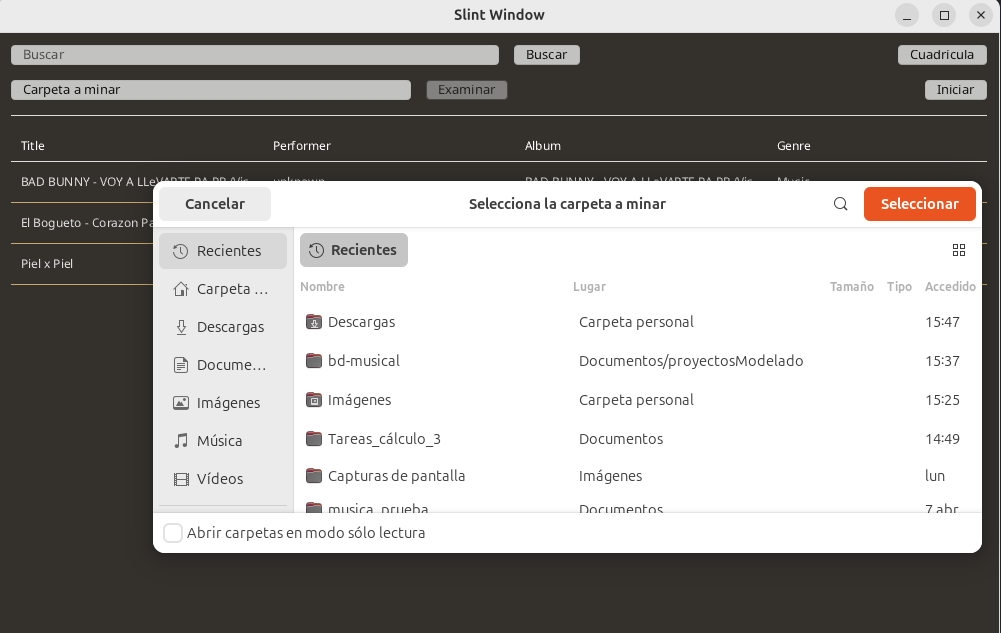
\includegraphics[width=0.8\textwidth]{img_resultados/minar} 
    \caption{Selección de carpeta}
\end{figure}
\begin{figure}[h]
    \centering
    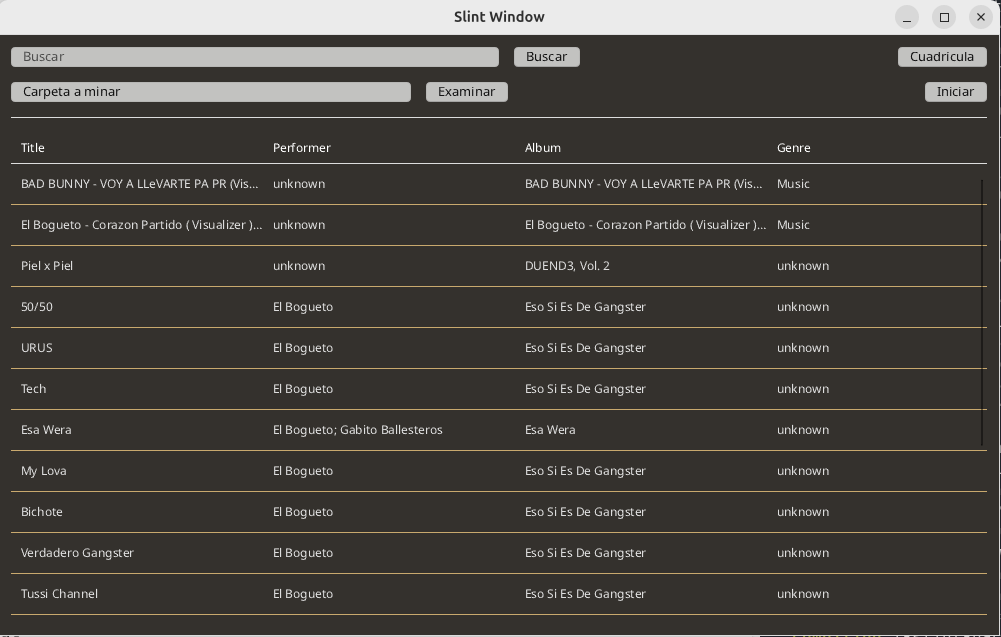
\includegraphics[width=0.8\textwidth]{img_resultados/resultado} 
    \caption{Carpeta minada}
\end{figure}
\begin{figure}[h]
    \centering
    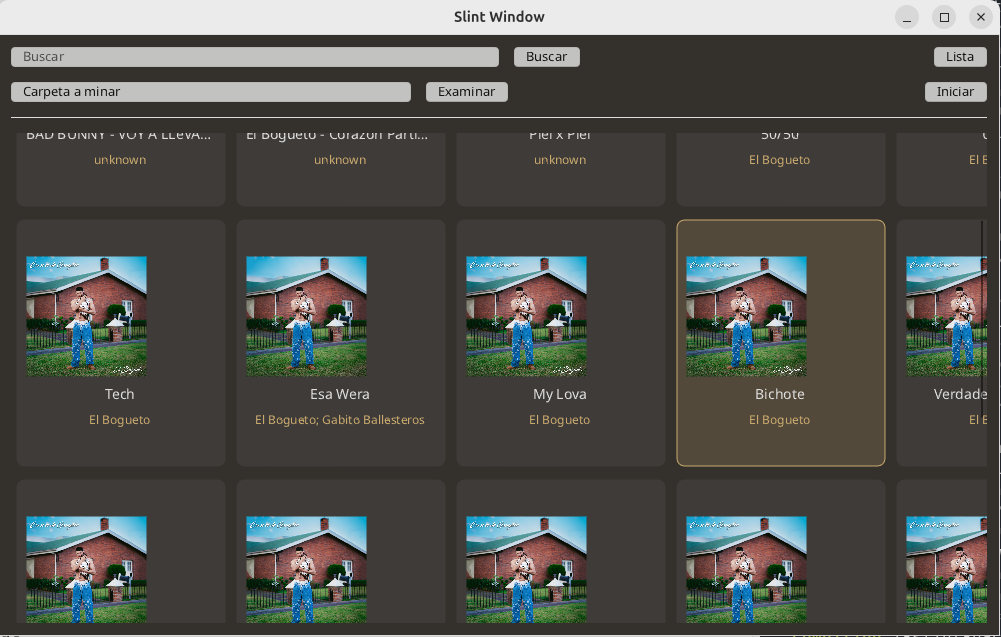
\includegraphics[width=0.8\textwidth]{img_resultados/cuadricula} 
    \caption{Vista cuadricula}
\end{figure}
\begin{figure}[h]
    \centering
    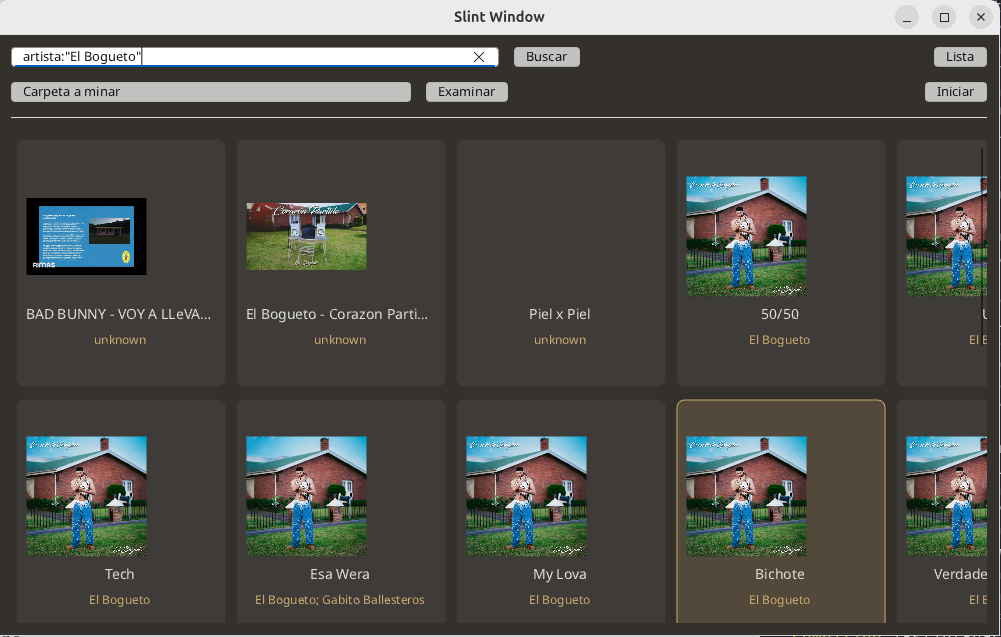
\includegraphics[width=0.8\textwidth]{img_resultados/buscar} 
    \caption{Búsqueda}
\end{figure}
\begin{figure}[h]
    \centering
    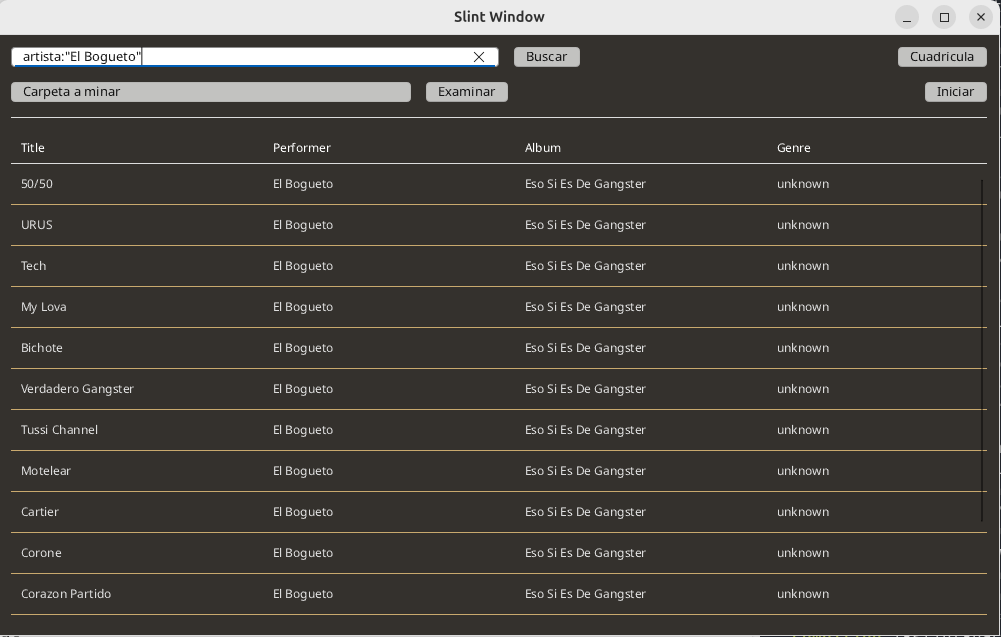
\includegraphics[width=0.8\textwidth]{img_resultados/busqueda_lista} 
    \caption{Resultados de la búsqueda}
\end{figure}

\clearpage

\section{Conclusiones}
A lo largo de este proyecto aprendí a manejar distintas herramientas que no había utilizado anteriormente, también
trabajado con interfaces cosa que no había hecho, pude aprender a como manejar el estado y distintas cosas, sin
embargo también a tomar en cuenta el tiempo de entrega y cual debe ser el avance adecuado para poder realizar
una entrega en condiciones ya que muchas partes de este proyecto no obtuvieron el resultado que me hubiera gustado.

\section{Trabajo a Futuro}
Sería adecuado manejar de mejor manera los errores que puedan entregar algunas funciones ya que básicamente no se manejan,
también el estructurar de mejor manera los componentes de la interfaz y añadir lo necesario para poder
correr en docker.

\end{document}
